\subsubsection{IP Adressen}
Auf dem Backbone Router wurden die Adressen mit ``no ip address'' und ``no ipv6 address xxxx'' entfernt.\\
Bei den neuen Routern wurde auch IPv6 unicasting aktiviert.
Die LAN IPv6 werden mit `` ipv6 address 2x:x:x:x::x/64'' auf dem Interface konfiguriert.\\
Die WAN IPv6 wurden im ``conf t'' wie folgt aktiviert:\\
int gigx/x; ipv6 enable; ipv6 address fe80::x link-local;
\begin{figure}[!htb]
    \centering
    \begin{subfigure}{.49\textwidth}
        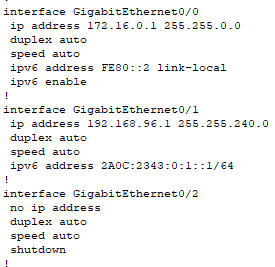
\includegraphics[width=\textwidth,height=.75\textwidth,keepaspectratio]{./ip/router1.png}
        \caption{Router 1}
    \end{subfigure}
    \begin{subfigure}{.49\textwidth}
        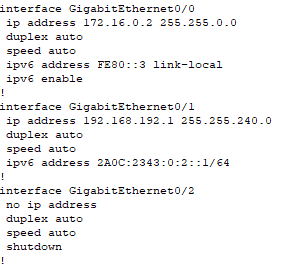
\includegraphics[width=\textwidth,height=.75\textwidth,keepaspectratio]{./ip/router2.png}
        \caption{Router 2}
    \end{subfigure}
    ~
    \begin{subfigure}{.5\textwidth}
        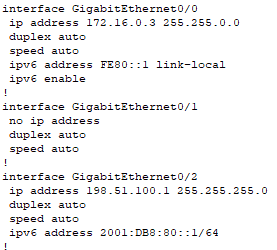
\includegraphics[width=\textwidth,height=.75\textwidth,keepaspectratio]{./ip/bbrouter.png}
        \caption{Backbone Router}
    \end{subfigure}
    \caption{Config nach den Änderungen}
\end{figure}
\FloatBarrier

\subsubsection{Routen}
Die IP Routes wurden wie folgt konfiguriert.
\paragraph{IPv4}
BB Router:
\begin{lstlisting}
Switch>en
Switch#conf t
Switch(config)#ip route 192.168.96.0 255.255.240.0 172.16.0.1
Switch(config)#ip route 192.168.192.0 255.255.240.0 172.16.0.2 
\end{lstlisting}
\begin{figure}[!htb]
    \centering
    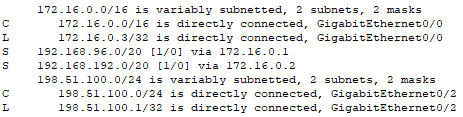
\includegraphics[width=\textwidth,height=.75\textwidth,keepaspectratio]{./routing/ipv4_bb.png}
    \caption{Routing Tabelle}
\end{figure}

\noindent
Router 1:
\begin{lstlisting}
Switch>en
Switch#conf t
Switch(config)#ip route 0.0.0.0 0.0.0.0 172.16.0.3
Switch(config)#ip route 192.168.192.0 255.255.240.0 172.16.0.2 
\end{lstlisting}
\begin{figure}[!htb]
    \centering
    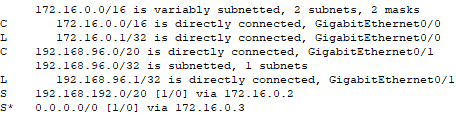
\includegraphics[width=\textwidth,height=.75\textwidth,keepaspectratio]{./routing/ipv4_1.png}
    \caption{Routing Tabelle}
\end{figure}

\noindent
Router 2:
\begin{lstlisting}
Switch>en
Switch#conf t
Switch(config)#ip route 0.0.0.0 0.0.0.0 172.16.0.3
Switch(config)#ip route 192.168.96.0 255.255.240.0 172.16.0.1
\end{lstlisting}
\begin{figure}[!htb]
    \centering
    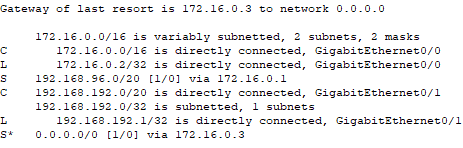
\includegraphics[width=\textwidth,height=.75\textwidth,keepaspectratio]{./routing/ipv4_2.png}
    \caption{Routing Tabelle}
\end{figure}

\paragraph{IPv6}
BB Router:
\begin{lstlisting}
Switch>en
Switch#conf t
Switch(config)#ipv6 route 2A0C:2343:0:1::/64 GigabitEthernet0/0 
FE80::2
Switch(config)#ipv6 route 2A0C:2343:0:2::/64 GigabitEthernet0/0 
FE80::3
\end{lstlisting}
\begin{figure}[!htb]
    \centering
    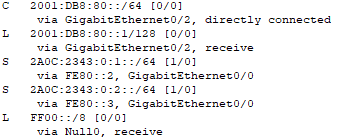
\includegraphics[width=\textwidth,height=.75\textwidth,keepaspectratio]{./routing/ipv6_bb.png}
    \caption{Routing Tabelle}
\end{figure}

\noindent
Router 1:
\begin{lstlisting}
Switch>en
Switch#conf t
Switch(config)#ipv6 route ::/0 GigabitEthernet0/0 FE80::1
Switch(config)#pv6 route 2A0C:2343:0:2::/64 GigabitEthernet0/0
FE80::3
\end{lstlisting}
\begin{figure}[!htb]
    \centering
    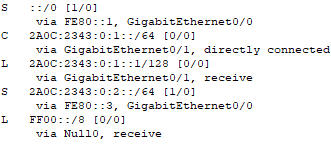
\includegraphics[width=\textwidth,height=.75\textwidth,keepaspectratio]{./routing/ipv6_1.png}
    \caption{Routing Tabelle}
\end{figure}

\noindent
Router 2:
\begin{lstlisting}
Switch>en
Switch#conf t
Switch(config)#ipv6 route ::/0 GigabitEthernet0/0 FE80::1
Switch(config)#ipv6 route 2A0C:2343:0:1::/64 GigabitEthernet0/0
FE80::2
\end{lstlisting}
\begin{figure}[!htb]
    \centering
    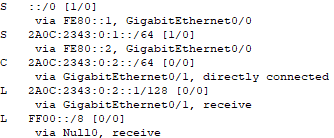
\includegraphics[width=\textwidth,height=.75\textwidth,keepaspectratio]{./routing/ipv6_2.png}
    \caption{Routing Tabelle}
\end{figure}

\paragraph{Interpretation der Tabellen}
Die Tabellen zeigen vor jeder Adresse immmer einen Buschstaben, der jeweils für etwas steht. C bedeutet, dass diese Adresse(Interface) verbunden ist. Mit L wird angegeben, dass es Lokal ist. MIt S werden die statischen Adressen verdeutlicht.\\
Unter der jeweiligen Adresse steht dann die Verbindungsart. Diese ist bei statischen immer eine Adresse und bei link-lokalen ist auch das Interface dabei.
Bei automatischen Adresserkennungen steht immer das Interface und dessen Funktion bzw. wie es verbunden ist. IPv4 kann auch die Anzahl der Masken und Subnetze enthalten.